\documentclass[review]{elsarticle}

\usepackage{lineno,hyperref}
\usepackage{siunitx}
\usepackage{glossaries}
\usepackage{booktabs}
\usepackage[super]{nth}
\usepackage{caption}
\usepackage[version=4]{mhchem}
\usepackage{paralist}
\usepackage{lastpage}
\usepackage{fancyhdr}
\usepackage[left=3.3cm,right=3.3cm,top=3.7cm,bottom=3.7cm,headheight=23pt]{geometry}
\usepackage[nodayofweek,level]{datetime}

\newcommand{\dc}{\formatdate{21}{3}{2017}}
\newcommand{\lud}{\formatdate{21}{3}{2017}}

\modulolinenumbers[5]

\makeglossaries

\bibliographystyle{elsarticle-num}

\makeatletter
\def\ps@pprintTitle{%
 \let\@oddhead\@empty
 \let\@evenhead\@empty
 \def\@oddfoot{}%
 \let\@evenfoot\@oddfoot}
\makeatother


\graphicspath{{images/}}

\pagestyle{fancy}
\fancyhf{}


\renewcommand{\headrulewidth}{0.5pt}
\renewcommand{\footrulewidth}{0.5pt}

\lhead{Anjo Weichbrodt \\ last update: \lud}
\chead{}
\tiny
\rhead{\textit{Creating a mock--up of a lime--based paint Layer \\to simulate readhesion interventions}}
\lfoot{2017\_MockUp\_PaintLayer.pdf}
\cfoot{}
\rfoot{Page \thepage\ de~\pageref{LastPage}}


\begin{document}

\begin{frontmatter}

\title{Creating a mock--up of a lime--based paint Layer to simulate readhesion interventions\tnoteref{t1}}
\tnotetext[t1]{date created: \dc \hspace*{1cm}last update: \lud \hspace*{1cm} document URL: \url{https://github.com/anjoweichbrodt/2017_MockUp_PaintLayer}}

\author{Anjo Weichbrodt}

\address{anjo.weichbrodt@gmail.com}

\newacronym{pmma}{PMMA}{polymethyl methacrylate}
\newacronym{hdpe}{HDPE}{high-density polyethylene}
\newacronym{pet}{PET}{polyethylene terephthalate}
\glsunsetall{}


\begin{abstract}
This document describes the creation of mock--up lime--based paint layer.
It has been used by the author in the past to simulate readhesion interventions.
A lime slurry is filled into prepared flat moulds and is set to carbonate in controlled environmental conditions.
The descriptions is optimized for paint layer flakes of \SI[product-units = single]{5 x 5 x 0.05}{\cm}.
The work is executed on a \gls{pmma} surface on which two groups of four flakes each are produced.
The preparation of the flakes and manipulation within the experiments requires some manual skill.
Four weeks should be allocated to the preparation.
\end{abstract}

\begin{keyword}
{mock--up lime--based paint layer}\sep{simulate readhesion interventions}
\end{keyword}

\end{frontmatter}

\linenumbers{}


\section{Material list}

\begin{inparaenum}[(1)]
  \item \gls{pmma} plate \SI{0.5}{\cm},
  \item \gls{pmma} plate \SI{0.2}{\cm},
  \item sheet of \gls{hdpe} with \SI{0.05}{\cm} or preferred layer thickness,
  \item \gls{pet} film,
  \item double--sided adhesive,
  \item slake lime,
  \item \ce{CaCO3}--powder,
  \item water sprayer,
  \item climate chamber or air tight boxes and \ce{K2SO4}, \ce{NaCl}, solid \ce{CO2}

\end{inparaenum}


\section{Mould}

Any plane glass--like surface can be used as mould support.
A \gls{pmma} plate of a thickness of \SI{0.5}{\cm} has proven to be both sturdy enough and relatively easy to score and break to the right size.
The \gls{pmma} plate is scored on lines, dividing the plate in \SI{15}{\cm} wide elements.
A clean break can be obtained by placing the scored line on a bevel and applying uniform force parallel to the line.
Those elements are then divided in \SI{27}{\cm} intervals using the same separating technique to obtain \SI[product-units = single]{15 x 27 x 0.5}{\cm} pieces.

Water is sprayed on the platform surface.
Benefiting from the high surface tension of water, a \gls{pet} film is then `coated' on to it.
The air bubbles between the \gls{pmma} plate and \gls{pet} film are eliminated from the center to the border by means of a brush.

In the next step, a sheet of \gls{hdpe} with a material thickness of \SI{0.05}{\cm} is cut into \SI{1}{\cm} wide strips.
The strips are further divided into \SI{25}{\cm} and \SI{11}{\cm} long elements.
For each mould support, 2 long strips and 3 short strips are needed.

Double--sided adhesive tape is now applied to one side of the strips.
The first \SI{25}{\cm} long strip is adhered on the \gls{pet}--`coated' \gls{pmma} board.
Following the 3 shorter elements are attached perpendicular to it: one at each end and one in the middle.
The second \SI{25}{\cm} strip is adhered parallel to the first one at the other end of the small elements.
Thus, two empty squares of \SI[product-units = single]{11 x 11}{\cm} are created.
The result of this procedure is llustrated in Figure~\ref{fig:mould}.

\begin{figure}[htb]
\centering
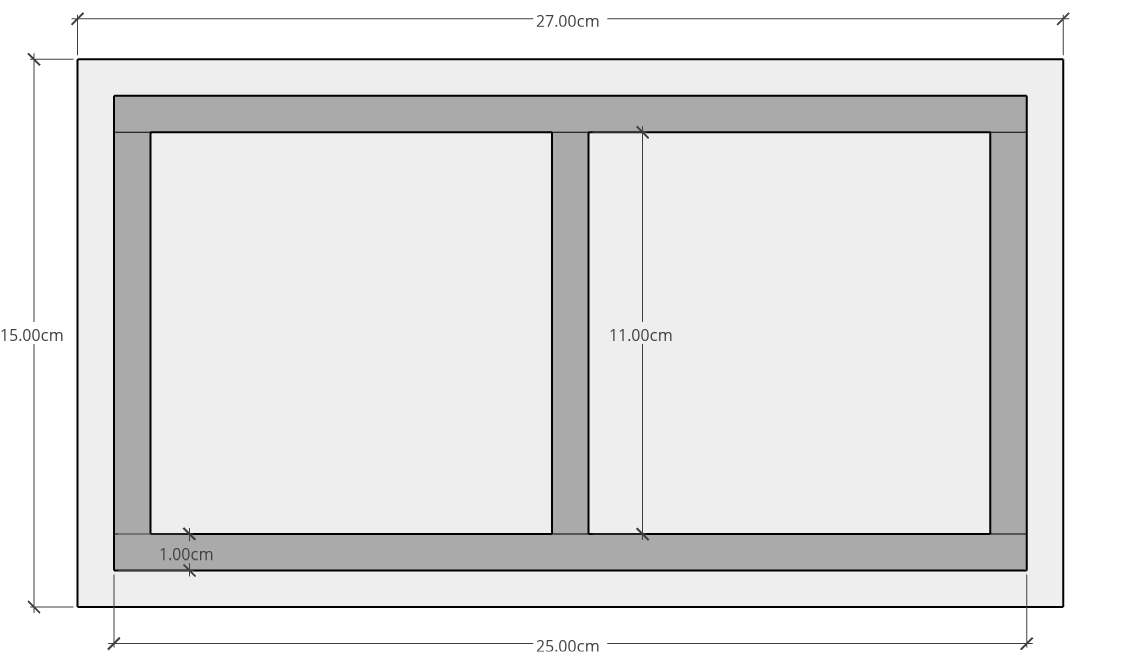
\includegraphics[width=\textwidth]{mould}
\caption{Drawing of the mould. Light grey: \gls{pmma} board with `coating'. Dark grey: \gls{hdpe} strips adhered with double sided adhesive tape.}
\label{fig:mould}
\end{figure}


\section{Material preparation}

Two parts of \ce{CaCO3}--powder,
0.1 parts of yellow ochre and 1 part of slaked lime are mixed together for \SI{10}{\minute} using a trowel.
No additional water is needed.
The lime paste is applied in the squares of the moulds, starting from the center and then dragging the material to the borders.
For this part a wide trowel, covering the span of the mould, works best.
Holding the trowel at a low angle and letting it slide on the mould border will level the material to a height of \SI{\approx0.05}{\cm}.


\section{Conditioning}

Once a mould is finished it should be quickly be inserted into a high humidity environment of \SI{\approx95}{\percent}.
If a climate chamber is not available for this purpose, the moulds can be placed in a closed box containing a \ce{K2SO4} brine, thus creating a relative humidity of \SI{\approx97}{\percent} at \SI{20}{\celsius}.
This humid environment conditioning should ideally last 2--5 days to allow for a slower loss of water without causing cracking.
Carbonation is not favored in those conditions.
Therefore, after the initial settling time the moulds are taken to a lower relative humidity of \SI{\approx65}{\percent}.
This phase needs particular care in the beginning:
Whenever the surface shows signs of drying, such as the brightening of surface color, it should be moistened with a fine water haze using a well--functioning water sprayer.
The first 8 hours in \SI{\approx65}{\percent} relative humidity are the most critical for avoiding cracking.
In the following days, water spraying can be reduced slowly and finally stoped.
moulds are left in these conditions for 3 weeks to allow carbonation of the specimen.
If a climate chamber is not available, a \ce{NaCl} brine can be used in a closed box to create a relative humidity of \SI{\approx75.5}{\percent} at \SI{20}{\celsius}.
In this case some dry ice (solid \ce{CO2}) should be placed in the box to provide the required \ce{CO2} for the carbonation process (\SI{100}{\g} dry ice sublime to \SI{\approx54}{\l} gaseous \ce{CO2}).
Using a high \ce{CO2} environment will reduce the time required for carbonation of the specimen.


\section{Flake separation}

During the last step, lime--based paint layers measuring \SI[product-units = single]{11 x 11}{\cm} are divided into four squared flakes with dimensions of \SI[product-units = single]{5 x 5 x 0.05}{\cm}.
In order to work efficiently without breaking the fragile \ce{CaCO3}--plates, a set of stencils can be used made from the \SI{0.2}{\mm} \gls{pmma} board.

\begin{figure}[htb]
  \centering
  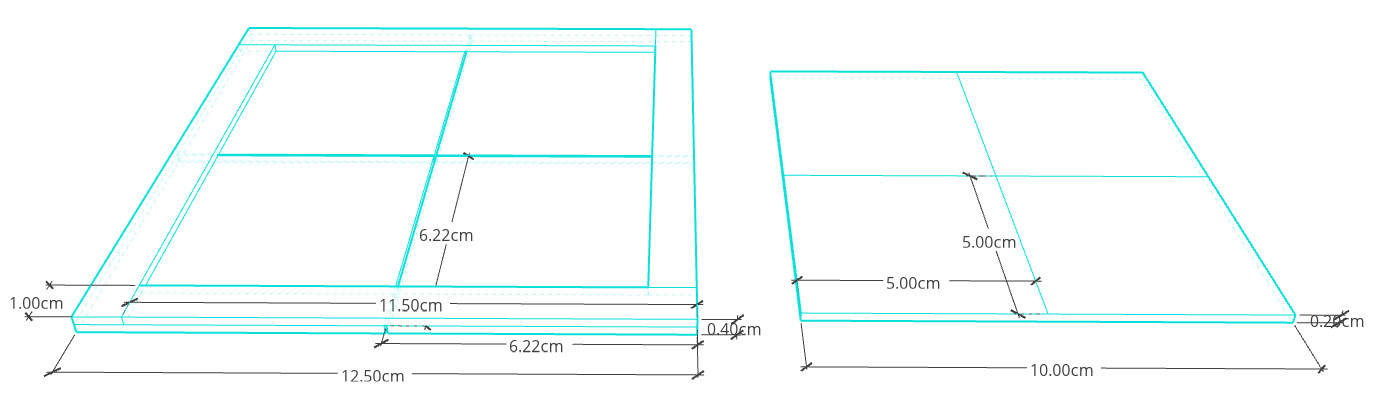
\includegraphics[width=\textwidth]{stencil_00}
  \caption{(Left) Stencil used to cut the line in between the flakes. (Right) Stencil used to cut the outlines of the flakes.}
  \label{fig:stencil_00}
\end{figure}

The first stencil, used to cut the line in between the flakes, is composed of four \SI[product-units = single]{6.2 x 6.2}{\cm} squares, glued to a frame forming a large square leaving slight space in between each other (Figure~\ref{fig:stencil_00} left).
The second element, used to cut the outlines of the flakes, is a simple \SI[product-units = single]{10 x 10}{\cm} square with a scored target cross centered at its middle (Figure~\ref{fig:stencil_00} right).
The first element is applied in the middle of the lime--based paint layer.
With a scalpel lines are scored in the space between the \gls{pmma} squares (Figure~\ref{fig:scoring_01}).
The second stencil element is now positioned on the newly--scored target cross of the lime--based paint layer and the outer lines are scored with the scalpel (Figure~\ref{fig:scoring_02}).

\begin{figure}[htb]
  \centering
  \begin{minipage}[t]{0.48\textwidth}
  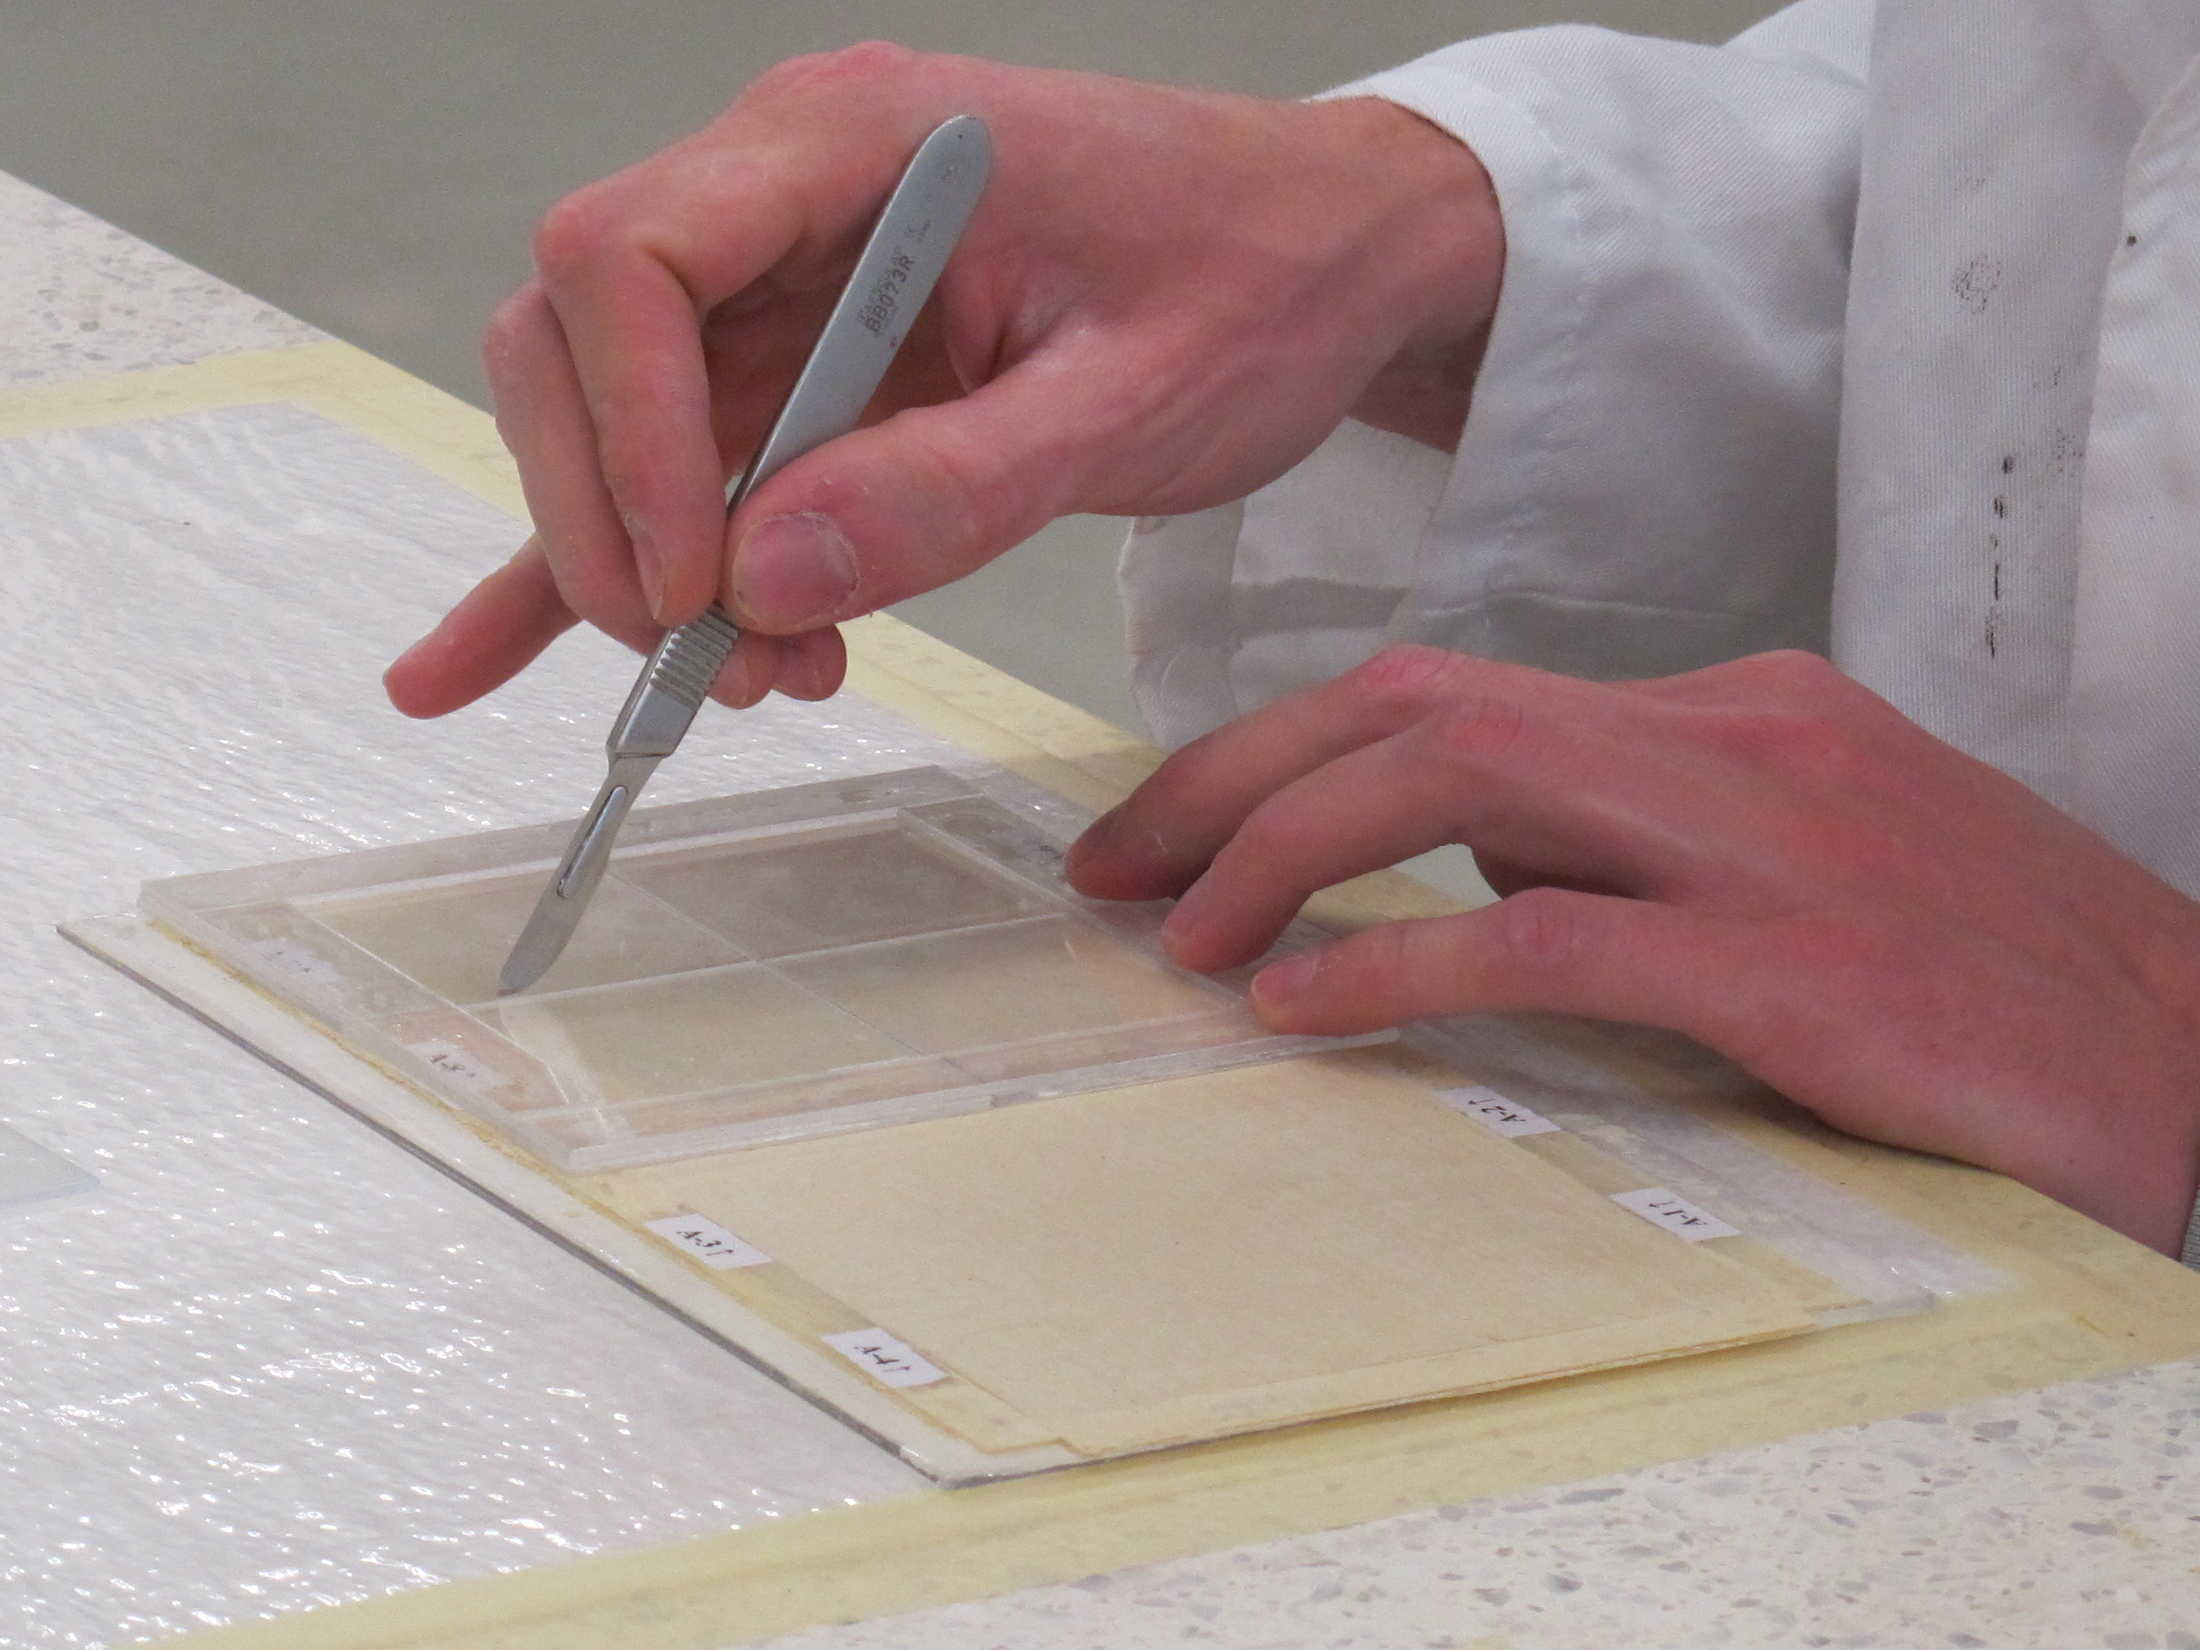
\includegraphics[width=\textwidth]{scoring_01}
  \caption{Scoring of the lime--based paint layer (inner lines).}
  \label{fig:scoring_01}
  \end{minipage}
  \hfill
  \begin{minipage}[t]{0.48\textwidth}
  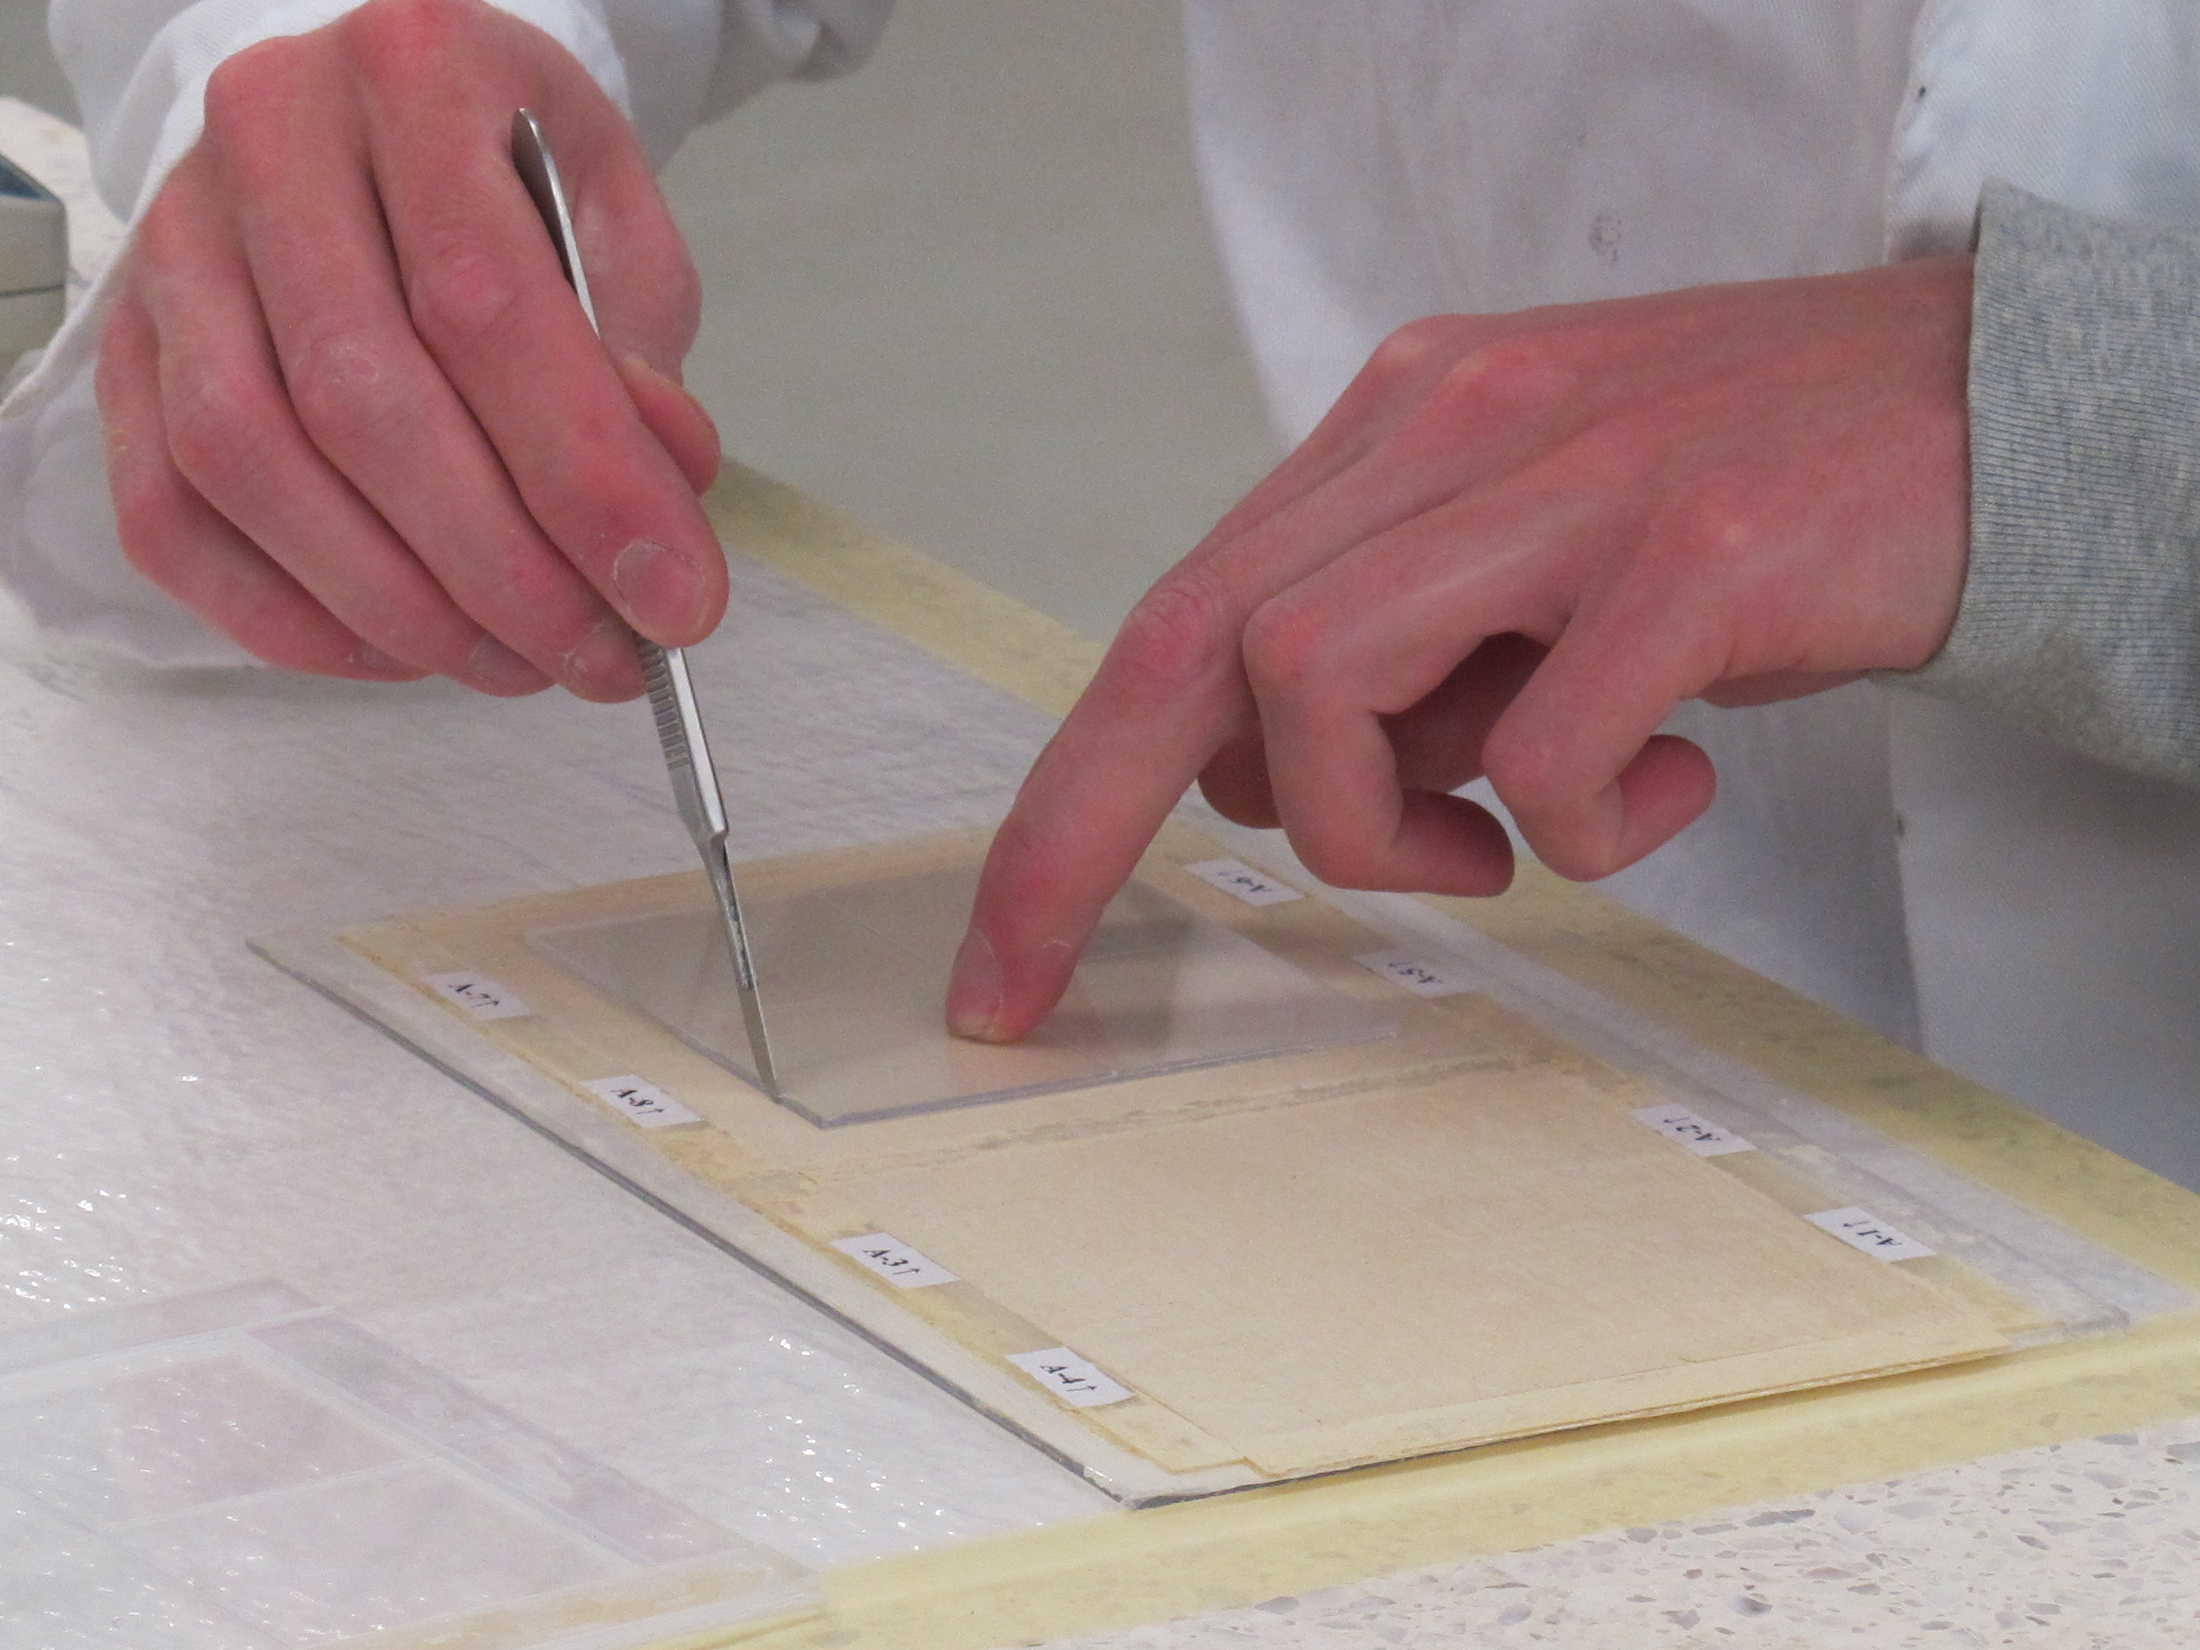
\includegraphics[width=\textwidth]{scoring_02}
  \caption{Scoring of the lime--based paint layer (outer lines).}
  \label{fig:scoring_02}
  \end{minipage}
\end{figure}

The separation of the different flakes is the most difficult part of the process, as the thin and brittle material can easily be damaged.
To accomplish this the surrounding \ce{CaCO3}--material is first broken with the scalpel pressing the blade upright on the surface and freeing a \SI[product-units = single]{10 x 10}{\cm} main square.
The blade is then pressed carefully between the individual flakes to separate them.

\printglossary

\end{document}
